% --- SECTION 2 : LES TABLES ---
\section{Les Tables de plongée}

\begin{frame}{Introduction aux tables MN90 - FFESSM}
    \begin{itemize}
        \item \textbf{Origine :} Établies par la Marine Nationale en 1990 et adoptées par la FFESSM pour la plongée récréative.
        \item \textbf{Fondement scientifique :} Basées sur une modélisation du corps humain et des résultats statistiques d'expérimentations, à l'instar des tables de Haldane.
        \item \textbf{Modélisation des tissus :}
        \begin{itemize}
            \item Le corps est représenté par \textbf{12 compartiments fictifs}.
            \item Chaque compartiment a une capacité d'absorption ou d'élimination de l'azote équivalente aux tissus réels qu'il représente.
        \end{itemize}
        \item \textbf{Objectif :} Prévenir l'Accident de Désaturation (ADD) causé par la présence de bulles d'azote dans le corps.
    \end{itemize}
\end{frame}

\begin{frame}{Les Tables MN90 : de 6m à 22m}
    \begin{columns}[c]
        \column{0.4\textwidth}
        \begin{itemize}
            \item Lecture des paliers en fonction de :
            \begin{itemize}
                \item La \textbf{Profondeur} (m).
                \item La \textbf{Durée} de plongée (min).
            \end{itemize}
            \item Lecture de la \textbf{DTR} (Durée Totale de Remontée).
            \item Détermination du \textbf{GPS} (Groupe de Plongée Successive).
        \end{itemize}

        \column{0.6\textwidth}
        \begin{center}
            \vspace{-0.31cm}
            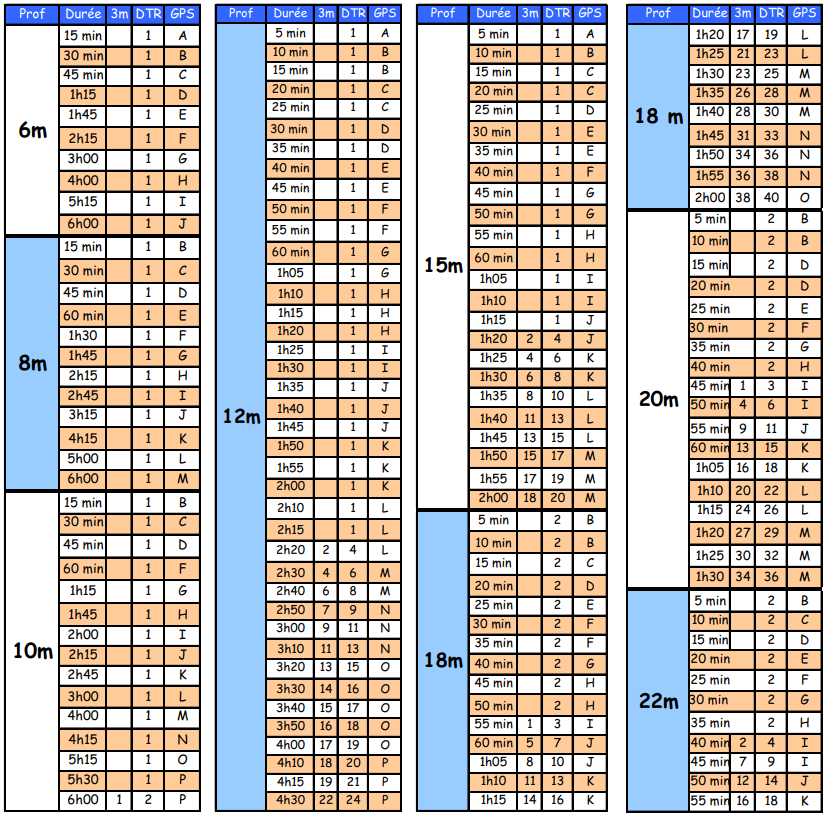
\includegraphics[height=0.9\textheight]{images/tables_mn90_6_a_22}
        \end{center}
    \end{columns}
\end{frame}

\begin{frame}{Les Tables MN90 : de 22m à 40m}
    \begin{columns}[c]
        \column{0.6\textwidth}
        \begin{center}
            \vspace{-0.32cm}
            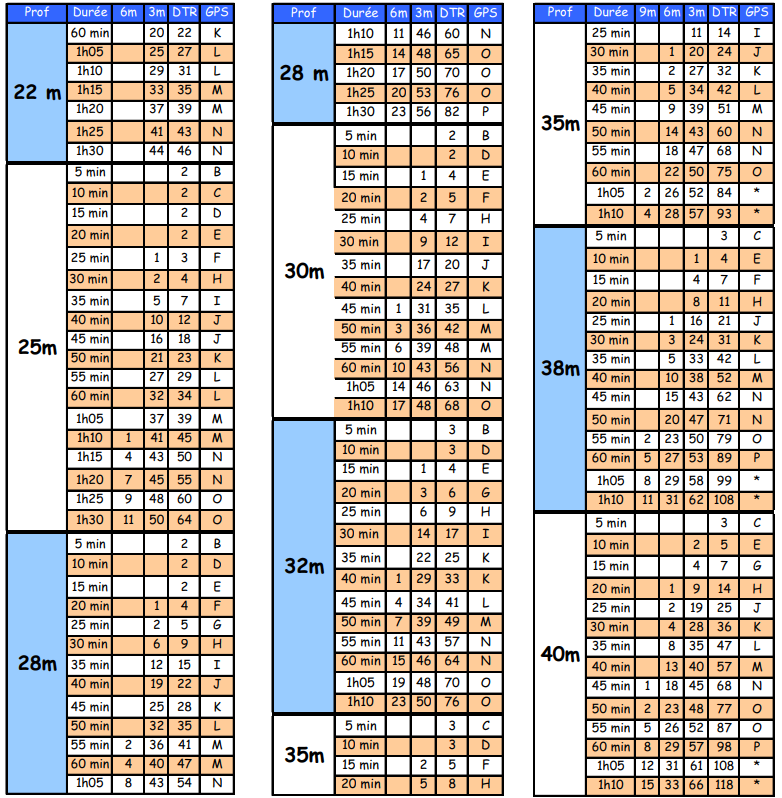
\includegraphics[height=0.9\textheight]{images/tables_mn90_22_a_40}
        \end{center}

        \column{0.4\textwidth}
        \begin{itemize}
            \item Apparition de paliers plus profonds (\textbf{6m} et \textbf{9m}) pour les immersions longues ou profondes.
        \end{itemize}
    \end{columns}
\end{frame}

\begin{frame}{Exemple d'application : Plongée simple}
    \begin{columns}[b]
        % Colonne Gauche : Le profil de plongée
        \column{0.45\textwidth}
        \begin{center}
            \vspace{-0.5cm}
            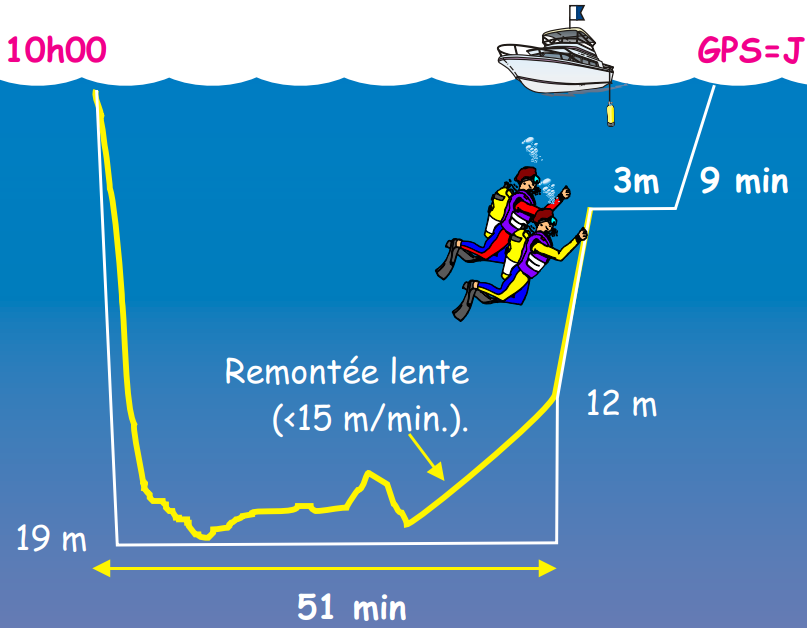
\includegraphics[width=0.9\textwidth]{images/plongee_simple}
            
            \begin{block}{Données de la plongée}
                \begin{itemize}
                    \item Profondeur max : \textbf{19 m}
                    \item Temps de plongée : \textbf{51 min}
                \end{itemize}
            \end{block}
        \end{center}

        % Colonne Droite : La lecture de table
        \column{0.52\textwidth}
        \textbf{Lecture dans la table MN90 :}
        \begin{itemize}
            \item Profondeur retenue : \textbf{20 m}
            \item Temps retenu : \textbf{55 min}
        \end{itemize}
        
        \begin{center}
            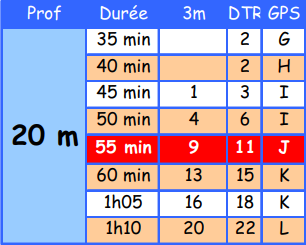
\includegraphics[width=0.45\textwidth]{images/tables_mn90_20}
        \end{center}
        \vspace{-0.3cm}
        \begin{alertblock}{Résultats}
            \begin{itemize}
                \item Palier à 3m : \textbf{9 minutes}
                \item DTR : \textbf{11 minutes} | GPS : \textbf{J}
            \end{itemize}
        \end{alertblock}
    \end{columns}
\end{frame}

\begin{frame}{Plongée consécutive ($< 15$ min)}
    \vspace{-0.2cm}
    \begin{columns}[c]
        \column{0.5\textwidth}
        \begin{center}
            \vspace{-0.3cm}
            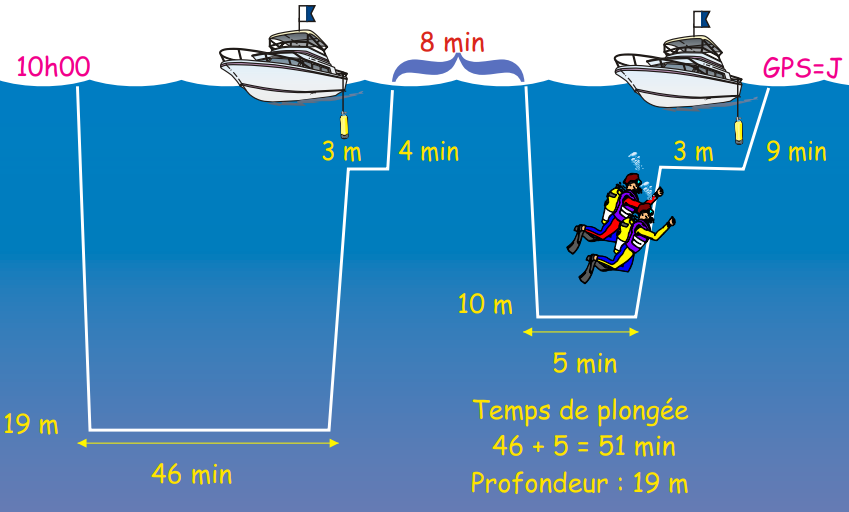
\includegraphics[width=\textwidth]{images/plongee_consecutive}
        \end{center}

        \vspace{-0.3cm}
        \begin{block}{Résultat final}
            \begin{itemize}
                \item Palier 3m : \textbf{9 min}
                \item GPS : \textbf{J}
            \end{itemize}
        \end{block}

        \column{0.48\textwidth}
        \begin{alertblock}{Règle de calcul}
            Si l'intervalle entre deux immersions est \textbf{inférieur à 15 minutes} :
            \begin{itemize}
                \item On considère qu'il s'agit de la \textbf{même plongée}.
                \item Profondeur : la plus \textbf{maximale} des deux.
                \item Temps : \textbf{somme} des durées des deux plongées.
            \end{itemize}
        \end{alertblock}
        \vspace{-0.3cm}
        \begin{center}
            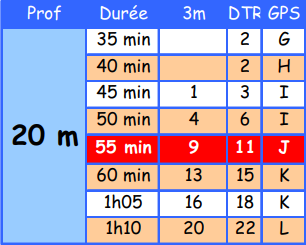
\includegraphics[width=0.45\textwidth]{images/tables_mn90_20}
        \end{center}
    \end{columns}
\end{frame}

\begin{frame}{Deux plongées par jour (Successives)}
    \begin{columns}[c]
        \column{0.5\textwidth}
        \begin{center}
            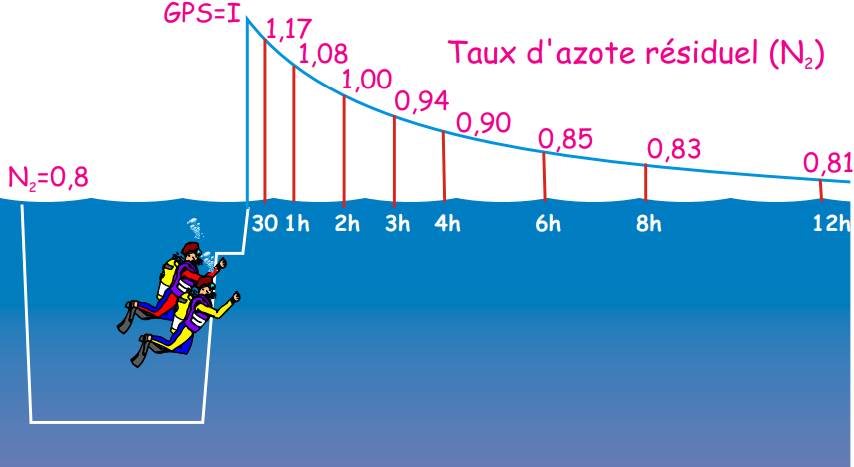
\includegraphics[width=0.95\textwidth]{images/plongee_successives_taux_n2}
        \end{center}
        \column{0.5\textwidth}
        \only<1>{
            \begin{block}{Le GPS (Groupe de Plongée Successive)}
                C'est une lettre qui représente la quantité d' \textbf{azote résiduel} restant dans l'organisme à la fin d'une plongée. 
            \end{block}
        }
        \only<2->{
            \begin{alertblock}{Règle de l'intervalle de surface}
                Pour le calcul de l'azote résiduel :
                \begin{itemize}
                    \item On utilise le tableau ci-dessous.
                    \item On prend toujours la valeur de \textbf{temps inférieure} la plus proche de l'intervalle réel.
                \end{itemize}
            \end{alertblock}
        }
    \end{columns}
    \vspace{-0.1cm}
    \begin{center}
        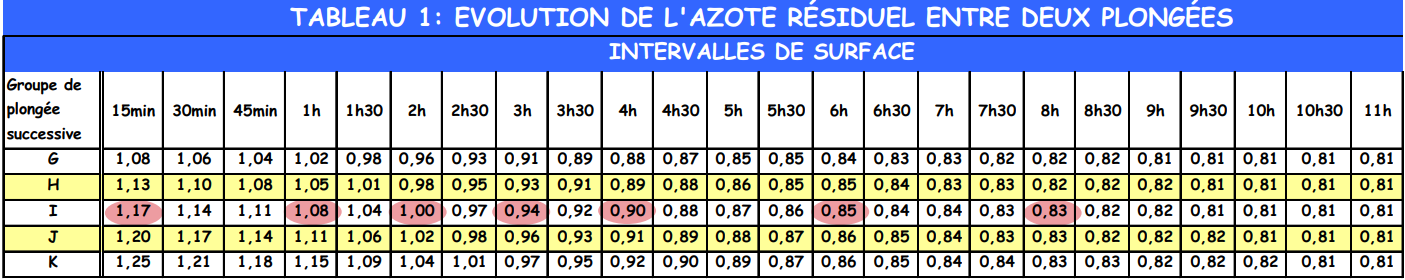
\includegraphics[width=0.9\textwidth]{images/tableau_n2}
    \end{center}
\end{frame}

\begin{frame}{Utilisation des tables : les paramètres clés}
    \begin{itemize}
        \item \textbf{Le profil "Carré" :} On considère que le plongeur est descendu immédiatement à la profondeur max et y est resté tout au long de l'immersion.
        \item \textbf{Profondeur à retenir :} On utilise toujours la \textcolor{ffessmred}{\textbf{profondeur maximale}} atteinte pendant la plongée.
        \item \textbf{Temps de plongée :}
        \begin{itemize}
            \item Il commence au \textcolor{ffessmred}{\textbf{début de la descente}}.
            \item Il s'arrête dès que le plongeur \textcolor{ffessmred}{\textbf{débute sa remontée}}
                 (vitesse préconisée entre \textcolor{ffessmred}{15 et 17m/min}).
        \end{itemize}
        \item \textbf{La remontée lente :} Si la vitesse est inférieure à 15m/min, le temps de remontée jusqu'au premier palier doit être \textbf{ajouté} au temps de plongée.
    \end{itemize}

    \begin{alertblock}{Principe fondamental des tables MN90}
        Les tables MN90 considèrent \textbf{toutes les plongées comme des plongées carrées} : le plongeur est supposé être resté à la profondeur maximale pendant toute la durée de l'immersion. C'est une approche \textbf{sécuritaire mais pénalisante}.
    \end{alertblock}
\end{frame}

\begin{frame}{Avantages et Limites des Tables}
    \begin{columns}
        \begin{column}{0.5\textwidth}
            \textbf{Avantages :}
            \begin{itemize}
                \item Fiabilité (pas de pile).
                \item Cadre rigoureux.
                \item Idéal pour la planification.
            \end{itemize}
        \end{column}
        \begin{column}{0.5\textwidth}
            \textbf{Limites :}
            \begin{itemize}
                \item Très pénalisantes (profil carré).
                \item Erreur humaine de lecture possible.
                \item Pas de calcul en temps réel si le profil change.
            \end{itemize}
        \end{column}
    \end{columns}
\end{frame}